\subsection{Euler and Kepler: Rotation Meets the Cosmos}

By the time Euler formalized the concept of \textbf{moment of inertia}, he wasn’t just helping physicists understand spinning tops or flywheels. He was laying the groundwork for a rotational understanding of planetary motion itself—including the insights at the heart of \textbf{Kepler’s Second Law}.

\subsubsection{The Moment of Area: A Rotational Parallel}

Recall Kepler’s Second Law: planets sweep out \textbf{equal areas in equal time}. That’s a statement about how angular motion varies with distance from the Sun. In Newton’s formulation, it’s explained as the consequence of a centripetal force acting through a central point—gravity tugging inward, and angular momentum conserved.

\begin{figure}[H]
\centering
\begin{tikzpicture}[scale=2.5, every node/.style={font=\small}]

  % Central body (Sun)
  \filldraw[yellow!80!orange] (0,0) circle (0.04);
  \node[below right=1pt] at (0,0) {\textbf{Sun}};

  % Orbit path
  \draw[thick,gray!60] (0,0) circle (1.1);

  % Two orbital positions
  \coordinate (A) at ({1.1*cos(30)}, {1.1*sin(30)});
  \coordinate (B) at ({1.1*cos(110)}, {1.1*sin(110)});
  \filldraw[blue] (A) circle (0.02);
  \filldraw[blue] (B) circle (0.02);

  \node[right=2pt] at (A) {\scriptsize Position 1};
  \node[left=2pt] at (B) {\scriptsize Position 2};

  % Central force vectors (gravity)
  \draw[->, thick, red!70!black] (A) -- ($(A)!0.3!(0,0)$);
  \draw[->, thick, red!70!black] (B) -- ($(B)!0.3!(0,0)$);

  \node at ($(A)!0.5!(0,0)+(0.05,-0.05)$) {\scriptsize $\vec{F}_{\text{gravity}}$};
  \node at ($(B)!0.5!(0,0)+(-0.1,0.05)$) {\scriptsize $\vec{F}_{\text{gravity}}$};

  % Equal area sweeps
  \fill[blue!20, opacity=0.4] (0,0) -- (A) arc[start angle=30, end angle=60, radius=1.1] -- cycle;
  \fill[blue!20, opacity=0.4] (0,0) -- (B) arc[start angle=110, end angle=140, radius=1.1] -- cycle;

  \node at (0.3,0.4) {\scriptsize Equal areas};

  % Caption
  \node at (0,-1) {
    \begin{minipage}{0.75\linewidth}
      \centering
      \footnotesize
      Newton explained Kepler’s Second Law through a central force: gravity pulls inward at all times, keeping the planet in orbit and ensuring that equal areas are swept out in equal time. The symmetry comes from the center—not rotation, but radial force.
    \end{minipage}
  };

\end{tikzpicture}
\caption{Newton’s interpretation of Kepler’s Second Law: planets sweep equal areas because of a centripetal force (gravity) acting through a fixed point—the Sun. The force is always radial, not rotational.}
\end{figure}


But Euler’s lens adds another twist:

\begin{quote}
What if the key quantity isn’t just area, or force—but how hard it is to \textit{change} the planet’s motion at any given radius?
\end{quote}

Enter the moment of inertia:

\[
I = \sum m r^2 \quad \Rightarrow \quad \text{or for continuous systems: } I = \int r^2 \, dm
\]

While Kepler was talking about sweeping areas, Euler would have looked at the \textbf{resistance to changing that sweep}—how much torque would be required to alter a planet’s path.


\begin{figure}[H]
\centering
\begin{tikzpicture}[scale=2.5, every node/.style={font=\small}]

  % Central mass (e.g., Sun)
  \filldraw[yellow!80!orange] (0,0) circle (0.04);
  \node[below right=1pt] at (0,0) {\textbf{Sun}};

  % Orbit ellipse (for simplicity, circle)
  \draw[thick,gray!60] (0,0) circle (1.1);

  % Two positions: closer and farther
  \coordinate (A) at ({1.1*cos(30)}, {1.1*sin(30)});
  \coordinate (B) at ({1.1*cos(120)}, {1.1*sin(120)});
  \filldraw[blue] (A) circle (0.02);
  \filldraw[blue] (B) circle (0.02);

  \node[right=2pt] at (A) {\scriptsize Position 1};
  \node[left=2pt] at (B) {\scriptsize Position 2};

  % Sector areas for equal time sweep
  \fill[blue!15, opacity=0.5] (0,0) -- (A) arc[start angle=30, end angle=60, radius=1.1] -- cycle;
  \fill[blue!15, opacity=0.5] (0,0) -- (B) arc[start angle=120, end angle=150, radius=1.1] -- cycle;

  \node at (0.5,0.4) {\scriptsize Equal areas};

  % Radius vectors
  \draw[->, thick] (0,0) -- (A);
  \draw[->, thick] (0,0) -- (B);

  \node at (0.3,0.85) {\scriptsize $r_1$};
  \node at (-0.8,0.6) {\scriptsize $r_2$};

  % Small mass elements at each position
  \draw[->, red!70!black, thick] (A) -- ++(60:0.3);
  \draw[->, red!70!black, thick] (B) -- ++(150:0.3);
  \node[red!70!black] at ($(A)+(60:0.3)+(0.15,0)$) {\scriptsize $m r_1^2$};
  \node[red!70!black] at ($(B)+(150:0.3)+(-0.2,0)$) {\scriptsize $m r_2^2$};

  % Label
  \node at (0,-1.0) {
    \begin{minipage}{0.75\linewidth}
      \centering
      \footnotesize Kepler said planets sweep out equal areas in equal time. Euler extended this thinking by introducing the moment of inertia: a measure of how hard it is to change that angular motion. The farther the mass is from the center, the more it resists — not linearly, but quadratically, as $I = \sum m r^2$.
    \end{minipage}
  };

\end{tikzpicture}
\caption{Kepler described how planets sweep equal areas in equal time. Euler’s moment of inertia added a deeper rotational insight: resistance to changing that sweep grows with $r^2$.}
\end{figure}



\subsubsection{From Kepler to Angular Momentum}

Using modern notation, Kepler’s Second Law implies conservation of angular momentum:

\[
L = I \omega = \text{constant}
\]

Where:
\begin{itemize}
    \item \( I = m r^2 \) is the moment of inertia (for a point mass),
    \item \( \omega = \frac{d\theta}{dt} \) is angular velocity,
    \item \( L \) is the angular momentum.
\end{itemize}

\begin{figure}[H]
\centering
\begin{tikzpicture}[scale=2.5, every node/.style={font=\small}]

  % Central body (e.g., Sun)
  \filldraw[yellow!80!orange] (0,0) circle (0.04);
  \node[below right=1pt] at (0,0) {\textbf{Sun}};

  % Orbit path (circular)
  \draw[thick,gray!60] (0,0) circle (1.1);

  % Planet position
  \coordinate (P) at ({1.1*cos(60)}, {1.1*sin(60)});
  \filldraw[blue] (P) circle (0.02);
  \node[above right=1pt] at (P) {Planet};

  % Radius vector r
  \draw[->, thick] (0,0) -- (P) node[midway, above left] {\scriptsize $r$};

  % Angular velocity arc
  \draw[->, thick,blue!60!black] (0.7,0) arc[start angle=0,end angle=60,radius=0.7];
  \node at (0.8,0.35) {\scriptsize $\omega = \frac{d\theta}{dt}$};

  % Angular momentum vector (perpendicular)
  \draw[->, thick,red!70!black] (P) -- ++(150:0.4);
  \node[red!70!black] at ($(P)+(150:0.45)$) {\scriptsize $L = I\omega$};

  % Inertia label
  \node at (-1.2,-0.7) {
    \begin{minipage}{0.7\linewidth}
      \centering
      \footnotesize Kepler’s equal-area law implies conservation of angular momentum. With $I = m r^2$ and $\omega = \frac{d\theta}{dt}$, we get $L = I\omega$, which stays constant as the planet orbits.
    \end{minipage}
  };

\end{tikzpicture}
\caption{Kepler's Second Law implies angular momentum is conserved: $L = I\omega = m r^2 \cdot \frac{d\theta}{dt}$. As the planet moves, $r$ and $\omega$ may change—but their product $L$ remains constant.}
\end{figure}


From this, we can derive Kepler’s area law:

\[
\frac{dA}{dt} = \frac{1}{2} r^2 \frac{d\theta}{dt} = \frac{L}{2m}
\]

This means:
- When the planet is closer to the Sun (\( r \) is small), \( \omega \) must be large.
- When it's farther away, it rotates more slowly.
- But in both cases, the \textbf{area swept per unit time stays constant}.

Kepler saw the geometry.  
Leibniz wrote the integral.  
Newton explained the force.  
\textbf{Euler explained the resistance.}


\begin{figure}[H]
\centering
\begin{tikzpicture}[scale=2.5, every node/.style={font=\small}]

  % Central body
  \filldraw[yellow!80!orange] (0,0) circle (0.04);
  \node[below right=1pt] at (0,0) {\textbf{Sun}};

  % Orbit path (circular)
  \draw[thick,gray!60] (0,0) circle (1.1);

  % Two positions: close and far
  \coordinate (P1) at ({1.1*cos(30)}, {1.1*sin(30)});
  \coordinate (P2) at ({1.1*cos(150)}, {1.1*sin(150)});
  \filldraw[blue] (P1) circle (0.02);
  \filldraw[blue] (P2) circle (0.02);
  \node[right=2pt] at (P1) {\scriptsize Closer};
  \node[left=2pt] at (P2) {\scriptsize Farther};

  % Radius vectors
  \draw[->, thick] (0,0) -- (P1) node[midway, above right] {\scriptsize $r_1$};
  \draw[->, thick] (0,0) -- (P2) node[midway, above left] {\scriptsize $r_2$};

  % Angular velocity arrows
  \draw[->, red!70!black, thick] (P1) -- ++(120:0.3);
  \draw[->, red!70!black, thick] (P2) -- ++(210:0.15);
  \node[red!70!black] at ($(P1)+(120:0.35)$) {\scriptsize $\omega_1$ (fast)};
  \node[red!70!black] at ($(P2)+(210:0.35)$) {\scriptsize $\omega_2$ (slow)};

  % Equal area sectors
  \fill[blue!15, opacity=0.4] (0,0) -- (P1) arc[start angle=30, end angle=50, radius=1.1] -- cycle;
  \fill[blue!15, opacity=0.4] (0,0) -- (P2) arc[start angle=150, end angle=170, radius=1.1] -- cycle;

  \node at (0.2,0.3) {\scriptsize Equal areas swept};

  % Label
  \node at (0,-1.0) {
    \begin{minipage}{0.75\linewidth}
      \centering
      \footnotesize Kepler’s area law in modern form: $\displaystyle \frac{dA}{dt} = \frac{1}{2}r^2 \frac{d\theta}{dt} = \frac{L}{2m}$. \\
      Planets move faster when closer, slower when farther, but always sweep equal areas in equal time.
    \end{minipage}
  };

\end{tikzpicture}
\caption{Kepler’s Second Law as a statement of conserved angular momentum: $\frac{dA}{dt} = \frac{1}{2}r^2 \omega = \frac{L}{2m}$. The geometry hides a deep rotational symmetry.}
\end{figure}


\subsubsection{Why Euler's View Matters}

Euler didn’t reinterpret Kepler—he reinforced it by clarifying \textbf{what stays constant (angular momentum)} and \textbf{why}.

Unlike Newton’s triangles or Leibniz’s infinitesimals, Euler’s framework makes it clear that:
- Planetary motion isn’t just conserved geometrically or algebraically—it’s dynamically constrained by how mass behaves under rotation.
- This opens the door to generalizations: spinning tops, precessing orbits, gyroscopes, and eventually, relativity.

\subsubsection*{Diagram: Angular Momentum and Sweeping Areas}

\begin{figure}[H]
\centering
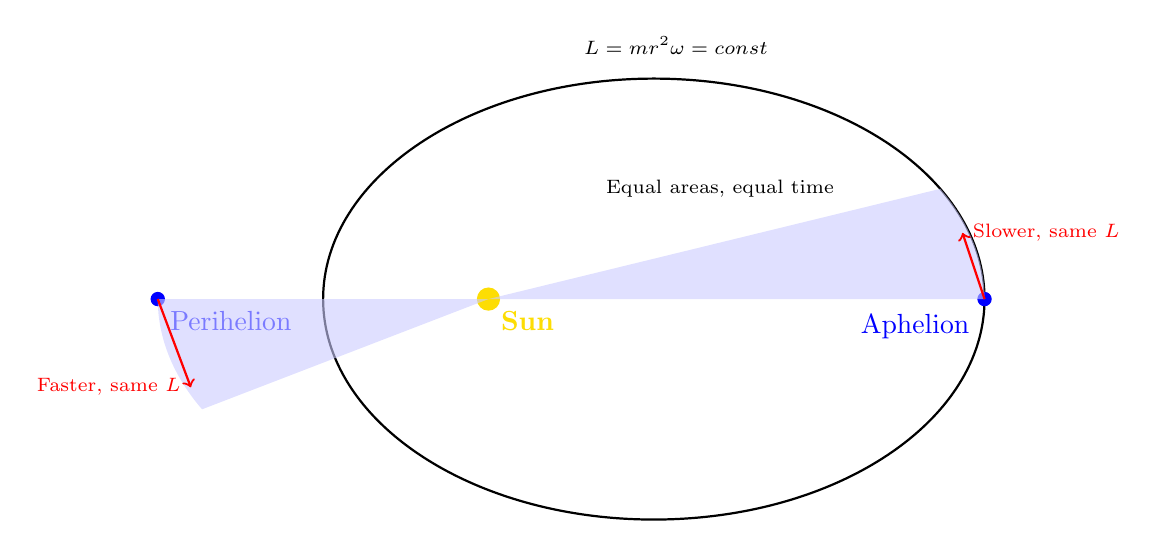
\begin{tikzpicture}[scale=2.8]
  % Elliptical orbit
  \draw[thick] (0,0) ellipse (1.5 and 1);

  % Sun at one focus
  \filldraw[yellow!80!orange] (-0.75,0) circle (0.05) node[below right=1pt] {\textbf{Sun}};

  % Aphelion and Perihelion
  \filldraw[blue] (1.5,0) circle (0.03) node[below left=2pt] {Aphelion};
  \filldraw[blue] (-2.25,0) circle (0.03) node[below right=1pt] {Perihelion};

  % Wedges for equal areas
  \fill[blue!20, opacity=0.6] 
    (-0.75,0) -- (1.5,0) arc[start angle=0,end angle=30,x radius=1.5cm, y radius=1cm] -- cycle;

  \fill[blue!20, opacity=0.6] 
    (-0.75,0) -- (-2.25,0) arc[start angle=180,end angle=210,x radius=1.5cm, y radius=1cm] -- cycle;

  % Angular momentum vectors
  \draw[->, red, thick] (1.5,0) -- (1.4,0.3) node[right] {\scriptsize Slower, same $L$};
  \draw[->, red, thick] (-2.25,0) -- (-2.1,-0.4) node[left] {\scriptsize Faster, same $L$};

  % Equation annotation
  \node at (0.1,1.15) {\scriptsize $L = m r^2 \omega = \text{const}$};

  % Label
  \node at (0.3,0.5) {\scriptsize Equal areas, equal time};

\end{tikzpicture}
\caption{Euler’s lens on Kepler’s law: Equal areas imply constant angular momentum, linking rotational inertia to orbital dynamics.}
\end{figure}

\subsubsection{The Chain of Insight}

\begin{center}
\begin{tikzpicture}[node distance=1.5cm and 2.8cm, every node/.style={align=center}]
\node (kepler) {\textbf{Kepler} \\ Geometry of Areas};
\node (leibniz) [below left=of kepler] {\textbf{Leibniz} \\ Infinitesimal Integrals};
\node (newton) [below right=of kepler] {\textbf{Newton} \\ Central Force, Geometry};
\node (euler) [below=of kepler] {\textbf{Euler} \\ Angular Momentum and Inertia};

\draw[->] (kepler) -- (leibniz);
\draw[->] (kepler) -- (newton);
\draw[->] (leibniz) -- (euler);
\draw[->] (newton) -- (euler);
\end{tikzpicture}
\end{center}

\begin{quote}
\textit{Kepler measured the sky. Newton explained the forces. Leibniz wrote the math. Euler made it move.}
\end{quote}




